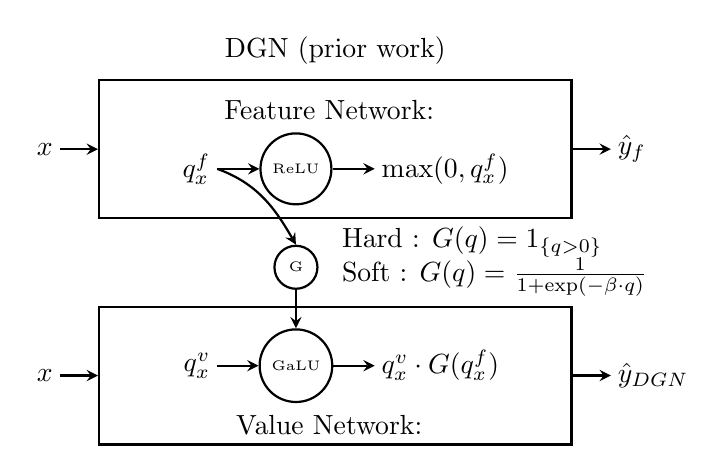
\begin{tikzpicture}

\node []  (fntext)at (3.5,1.5) {DGN (prior work)};
%Feature Network
\node [draw,
	minimum width=6cm,
	minimum height=1.75cm,
	thick
]  (fnbox)at (3.5,0.25) {};
\node []  (fntext)at (3.5,0.75) {Feature Network: $\Tf$};


%Feature Network Input
\node (fin) [left of=fnbox,node distance=3.5cm, coordinate] {};
\node[left=-1pt] at (fin.west){$x$};
\draw[-stealth, thick] (fin.center) -- (fnbox.west);

%Feature Network Output
\node (fout) [right of=fnbox,node distance=3.5cm, coordinate] {};
\node[right=-1pt] at (fout.west){$\hat{y}_{\text{f}}$};
\draw[-stealth, thick]  (fnbox.east)--(fout.center);


%ReLU Circle
\node[draw,
	circle,
	minimum size=0.75cm,thick,
] (relu) at (3,0){\tiny{ReLU}};
%ReLU Input
\node (b) [left of=relu,node distance=1cm, coordinate] {};

\node[left=-1pt] at (b.center){$q^\text{f}_x$};
\draw[-stealth, thick] (b.east) -- (relu.west);


%ReLU Output
\node (c) [right of=relu,node distance=1cm, coordinate] {};
\node[right=-1pt] at (c.center){$\max(0,q^\text{f}_x)$};
\draw[-stealth, thick] (relu.east) -- (c.west);
	

%Gating Circle
\node[draw,
	circle,
	minimum size=0.0625cm,thick,
] (gating) at (3,-1.25){\tiny{G}};
%\node[right=6pt] at (gating.north){Hard : $G(q)=\mathbbm{1}_{\{q>0\}} $};
%\node[below right=6pt] at (gating.north){Soft : $G(q)=\frac{1}{1+\exp(-\beta\cdot q)}$};

\node[right=6pt] at (3.25,-0.925){Hard : $G(q)=\mathbbm{1}_{\{q>0\}} $};
\node[right=6pt] at (3.25,-1.375){Soft : $G(q)=\frac{1}{1+\exp(-\beta\cdot q)}$};


%Value Network

\node [draw,
	minimum width=6cm,
	minimum height=1.75cm,
	thick
]  (vnbox)at (3.5,-2.625) {};

\node []  (vntext)at (3.5,-3.25) {Value Network: $\Tv$};

%Value Network Input
\node (vin) [left of=vnbox,node distance=3.5cm, coordinate] {};
\node[left=-1pt] at (vin.west){$x$};
\draw[-stealth, thick] (vin.center) -- (vnbox.west);

%Feature Network Input
\node (vout) [right of=vnbox,node distance=3.5cm, coordinate] {};
\node[right=-1pt] at (vout.west){$\hat{y}_{\text{DGN}}$};
\draw[-stealth, thick]  (vnbox.east)--(vout.center);



%GaLU Circle
\node[draw,
	circle,
	minimum size=0.75cm,thick,
] (galu) at (3,-2.5){\tiny{GaLU}};

\draw [-stealth,thick]   (b) to[out=-20,in=120] (gating.north);
\draw [-stealth,thick]   (gating.south) -- (galu.north);


%GaLU Input
\node (d) [left of=galu,node distance=1cm, coordinate] {};
\node[left=-1pt] at (d.center){$q^\text{v}_x$};
\draw[-stealth, thick] (d.east) -- (galu.west);
%GaLU Output
\node (e) [right of=galu,node distance=1cm, coordinate] {};
\node[right=-1pt] at (e.center){$q^\text{v}_x\cdot G(q^\text{f}_x)$};
\draw[-stealth, thick] (galu.east) -- (e.west);
	
\end{tikzpicture}

